\chapter{Performance and energy measurement}
\label{chap:medida}
\label{chap:rendimiento}

\section{What is being measured}

Before comparing results, keep the model, data and execution configuration fixed.
Also record the clock mode, mapping mode and number of repetitions.

\section{Latency measurement}

The tool measures the time taken by the model execution call. This includes
communication between the host and board, the SDK call and inference on the AKD1000.

File loading, model mapping and warm-up runs occur before measurement starts.

\begin{figure}[H]
  \centering
  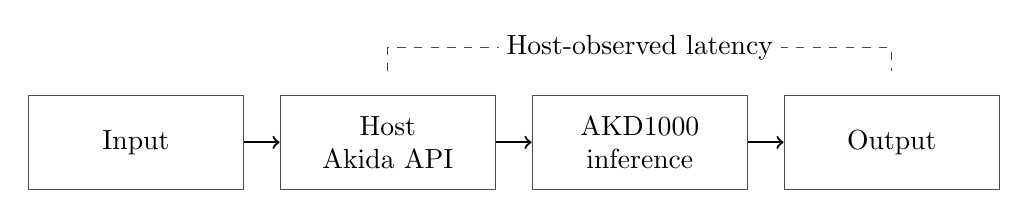
\begin{tikzpicture}[
    stage/.style={draw=black!70,align=center,
                  minimum height=12mm,text width=25mm,fill=white},
    flow/.style={->,thick,draw=black}
  ]
    \node[stage] (input) at (-4.8,0) {Input};
    \node[stage] (host) at (-1.6,0) {Host\\Akida API};
    \node[stage] (device) at (1.6,0) {AKD1000\\inference};
    \node[stage] (output) at (4.8,0) {Output};

    \draw[flow] (input) -- (host);
    \draw[flow] (host) -- (device);
    \draw[flow] (device) -- (output);

    \draw[dashed,black!70]
      (-1.6,0.9) -- (-1.6,1.2) -- (4.8,1.2) -- (4.8,0.9);

    \node[fill=white,inner sep=1mm] at (1.6,1.2)
      {Host-observed latency};
  \end{tikzpicture}

  \caption[Latency measurement boundary]
  {Elements included in the latency measurement from the host.}
  \label{fig:measurement-boundary}
\end{figure}

Results in this manual are therefore expressed as \emph{host-observed latency}.
They do not come from an isolated internal AKD1000 timer.

To measure the full execution time of an application, also include acquisition,
preprocessing and postprocessing.

\section{Run a benchmark}

Before a full campaign, run a short test to check the model, data and configuration.

\begin{lstlisting}[language=bash]
akd1000-bringup benchmark \
  --model models/model.fbz \
  --input data/inputs.npy \
  --method forward \
  --clock Performance \
  --map AllNps \
  --warmup 8 \
  --repetitions 1 \
  --output outputs/smoke
\end{lstlisting}

The output directory contains:

\begin{itemize}
  \item \code{latencies.csv}, with individual measurements;
  \item \code{summary.json}, with the configuration and trial summary;
  \item \code{host.json}, with information about the host used.
\end{itemize}

Check that the sample count, units and configuration are as expected. If the test
passes, repeat the benchmark with the required number of repetitions and save the
results in a different directory.

To compare configurations, change one variable at a time. For example, keep the model
fixed and compare \code{AllNps}, \code{HwPr} and \code{Minimal}, or keep the mapping
fixed and change the clock mode.

\section{Power and energy}

Akida can enable device power measurement and report statistics after inference
\cite{brainchip_akida_guide}:

\begin{lstlisting}[language=Python]
device.soc.power_measurement_enabled = True

model.forward(data)

print(model.statistics)
\end{lstlisting}

The power reported by this API is the measurement available on the device. It does
not represent the total consumption of the Raspberry Pi, carrier and board.

Given average power and host-observed latency, estimated energy per inference can be
calculated as

\begin{equation}
  E_{\mathrm{est}} \,[\mu\mathrm{J}]
  =
  P_{\mathrm{API}} \,[\mathrm{mW}]
  \,
  t_{\mathrm{host}} \,[\mathrm{ms}].
\end{equation}

The unit relationship is direct:

\[
1\,\mathrm{mW}\cdot 1\,\mathrm{ms}
=
1\,\mu\mathrm{J}.
\]

This estimate combines API power with host-observed latency. It helps compare runs
made with the same procedure; it measures neither internal chip energy nor total
system energy consumption.

Measuring total consumption would require external instrumentation on the assembly's
power supply.

\section{Save the results}

For each trial, retain at least:

\begin{itemize}
  \item the model and its version;
  \item the input data;
  \item the clock mode;
  \item the mapping mode;
  \item the number of repetitions;
  \item the files generated by the benchmark.
\end{itemize}

When comparing platforms such as CPU, GPU or FPGA, use the same task, data and an
equivalent measurement definition.
